\chapter{Online State Learning}
\section{Overview}

Although the offline state learning approach works for high-dimensional state problems, it has the shortcoming that it needs a database with images of the environment to work. This can be time consuming and not robust to changes in the environment. Thus, it would be desirable to have a version of D-COACH that eliminates the requirement of recording demonstrations and pre-training an autoencoder, learning everything in a single interaction step, as the original COACH does. Hence, an algorithm capable of training all the parameters of the network interactively from scratch. 

\section{D-COACH: Online State Learning}
In order to obtain an algorithm capable of learning everything from scratch interactively we need to make the networks converge faster. In the past chapter, an autoencoder was used to learn a low-dimensional representation of high-dimensional states in an offline learning process. In this chapter we propose to use the autoencoder learning criteria during the interactive learning process, such that both networks (the policy and the autoencoder) share the convolutional layers of the encoder, as shown in Fig.~\ref{fig:msim}.

\begin{figure}[H]
    \centering
    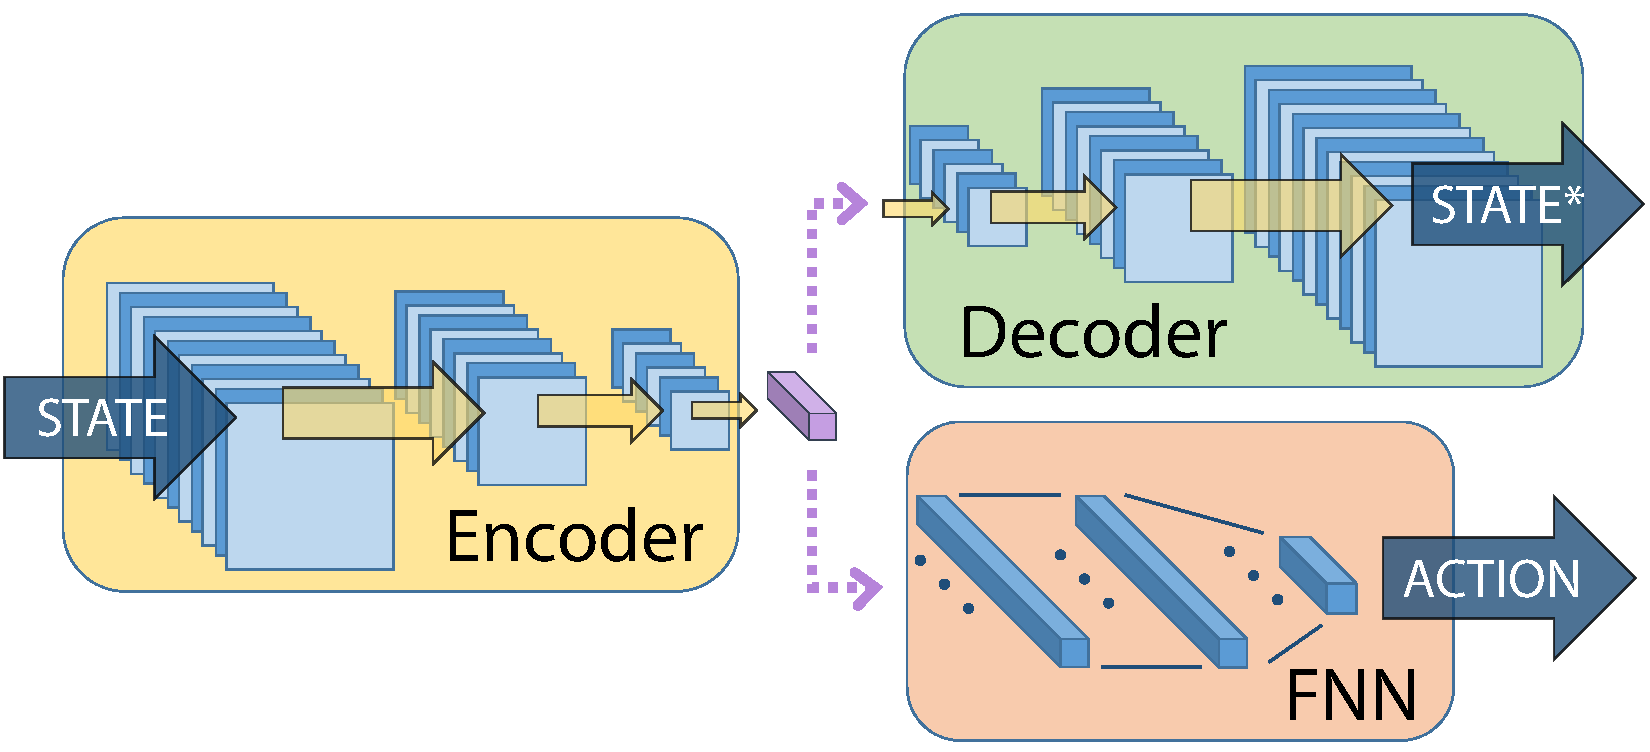
\includegraphics[width=0.6\linewidth]{imagenes/cap2/m2.pdf}
    \caption{D-COACH online state learning. The state representation is shared between the autoencoder and the policy training.}
    \label{fig:msim}
\end{figure}

The policy network has the convolutional layers at the input, followed by a second part that is a fully-connected layer, then this network maps from STATE to ACTION, while the autoencoder network involves the computation from STATE to STATE$^{*}$, wherein  STATE$^{*}$ is the reconstructed image at the output of the decoder.

In this case, the autoencoding is seen as an additional auxiliary criteria for training the state representation of the policy online. So, in addition to the loss function for predicting the policy based on the data generated by the human corrections, it also includes the loss function of the reconstruction at the output of the autoencoder, based on the same data stored during the human corrections. 

\section{The Algorithm}
Algorithm \ref{algorithm:EnDeepCOACH} describes the online state learning version of D-COACH. The algorithm first sets the hyper-parameters like the magnitude of the error \eqref{eq:error}, and the ones used for the corrections replay. Line 4 to 18 shows the algorithm that is executed every time step. In cases when the teacher advises a correction in line 6, the subsequent lines are evaluated, wherein the policy network is updated along with the autoencoder network, and the buffer of state-action pairs for the corrections replay process.

Two different updates are computed, one for the layers involved in the policy computation, and another for the layers of the autoencoder. When an advice of correction is given, the \textbf{update} \emph{policy} instruction updates the policy network for the current state and the \emph{batch\_update} subroutine is called. This subroutine updates the policy and the autoencoder using a mini-batch sampled from the replay buffer. If the reconstruction error of the autoencoder (difference between STATE and STATE$^{*}$) is greater than a threshold $\epsilon$ (line 6), the autoencoder is updated with the same mini-batch using the instruction \textbf{update} $AE$ (autoencoder). Otherwise, the convolutional layers are frozen, so that the instruction \textbf{update} \emph{policy} in lines 5 and 19, only modifies the non-convolutional layers with the Stochastic Gradient Descent (SGD) operation. The \emph{batch\_update} subroutine is also called every $b$ time steps (line 24).

 The \textbf{update} \emph{policy} instruction uses [state,$y_\mathrm{label}$] pairs (where $y_\mathrm{label(t)}=a_{t}+\mathrm{error_{t}}$), whereas \textbf{update} $AE$ only uses states. The aforementioned condition in line 6 is used for avoiding conflicts in the gradients of both cost functions, so when the latent vector of the AE is considered a good smaller representation of the state, the gradient of the policy must be prevented from harming the learned encoding. Hence, the encoder is kept frozen, unless unknown regions of the state space are visited. 


\begin{algorithm}[h]
\caption{D-COACH: online state learning}\label{algorithm:EnDeepCOACH}
\begin{algorithmic}[1]
\algdef{SE}[SUBALG]{Indent}{EndIndent}{}{\algorithmicend\ }%
\algtext*{Indent}
\algtext*{EndIndent}

\State \textbf{Require:} error magnitude $\textit{e}$, buffer update interval $b$, buffer sampling size $N$, buffer max. size $K$, buffer min. size $k$, pre-trained encoder parameters (if 3-step sequential learning) 
\State \textbf{Init:} $B = []$ \emph{\# initialize memory buffer}

\colorbox{lightgray}
{\parbox{\linewidth}{\State \textbf{function} batch\_update \emph{\# define batch update function}
\Indent
\If{$\mathrm{length}(B) \geq k$}
\State \textbf{update} \emph{policy} using SGD with a mini-batch sampled from $B$
\If{$AE_{\mathrm{error}}>\epsilon$}
\State \textbf{unfreeze} convolutional layers
\State \textbf{update} $AE$ using SGD with a mini-batch sampled from $B$
\Else
\State \textbf{freeze} convolutional layers
\EndIndent
\EndIf
\EndIf
}}
\colorbox{lightlightgray}{\parbox{\linewidth}{%
\For{t = 1,2,...}{} \emph{\# main loop}
\State \textbf{observe} state $s_{t}$
\State \textbf{execute} action $a_{t}=\pi(s_{t})$
\State \textbf{feedback} human corrective advice $h_{t}$
\If{$h_{t}$ is not \textbf{0}}
\State $\mathrm{error}_{t} = h_{t}\cdot e$
\State $y_{\mathrm{label}(t)} = a_{t} + \mathrm{error}_{t}$ 
\State \textbf{update} \emph{policy} using SGD with pair ($s_{t}$, $y_{\mathrm{label}(t)}$) 
\State \textbf{call} batch\_update
\State \textbf{append} $(s_{t}, y_{\mathrm{label}(t)})$ to $B$
\EndIf
\If{length($B$) $> K$ }
\State $B = B[2:K+1]$
\EndIf
\If{$\operatorname{mod}(t, b)$ is 0}
\State \textbf{call} batch\_update
\EndIf
\EndFor}}
\end{algorithmic}
\end{algorithm}

\section{Experiments and Results}

Three different types of experiments were carried out for validating this version of D-COACH: i) experiments with simulated teachers for evaluating the learning method under controlled conditions without influence of human factors, ii) validations with real human teachers, and iii) extra validations on real physical systems.

In these experiments we denote the enhanced D-COACH simply with `D-COACH', while from now on we call the previous version `basic D-COACH'. In the experiments, the learning processes are analyzed in three different problems:

\textbf{Car Racing:} A simulated problem (from OpenAI gym \cite{brockman2016openai}) in which the agent has to learn to drive from a top-down view of a racing car game (see Fig.~\ref{fig:Car_Racing}). The objective of the task is to drive a racetrack as fast as possible without leaving it. The default state that is given by the environment is a $96\times96\times3$ top-down view of the car which we downsampled to $64\times64\times1$. The continuous action space consists of 3 dimensions: \textbf{[direction, acceleration, brake]}. The \emph{direction} range goes from $-1$ to $1$, the \emph{acceleration} from $0$ to $1$ and the \emph{brake} from $0$ to $1$. In this problem, experiments with the simulated teacher and human teachers were carried out. The coupled feedback strategy was used in the experiments with human teachers, as presented in \cite{perez2018interactive}.

\begin{figure}[h]
    \centering
    \includegraphics[scale=0.8]{imagenes/cap3/car_racing_env.jpg}
    \caption{Car Racing, environment view.}
    \label{fig:Car_Racing}
\end{figure}
    
\textbf{Duckie Racing:} This is also a driving task, but in this case with a real/simulated robot which has an onboard camera that gives a first-person view of the environment. The real robot consist of a Duckiebot from the project Duckietown \cite{Paull2017}. The simulated robot is based on \cite{gym_duckietown}. A $120\times160\times3$ observation image is received from the environment which is downsampled to $64\times64\times1$. The same road was used for both the simulated and real robot. In the simulations, at the start of each episode, the robot can start, randomly, at the points A or B (plus random noise) of the map (see Fig.~\ref{fig:duckietown}). Each simulated episode lasts 1000 time steps (unless the robot leaves the road before) and as a performance metric a modified version of the default reward function of the environment is used, which has the following shape: $R = Cv\theta - Dd$. $C$ and $D$ are constants ($C=100$, $D=1$), $v$ is the linear velocity of the duckiebot, $\theta$ is its orientation with respect to $\gamma$ (a bezier curve that defines the path the agent is expected to follow) and $d$ is its distance to $\gamma$. The duckiebot is a differential robot, so the default actions consisted of speed commands ranging from -1 to 1 for each of the two wheels. To make it more intuitive for a human teacher to give feedback, the environment had an inverse kinematics module for the actions to be linear and rotational speeds instead, also ranging from -1 to 1. This problem is also used for experiments and validation with simulated and real human teachers.

\begin{figure}[h]
\centering
\subfloat[][Duckiebot.]{\includegraphics[width=0.305\linewidth]{imagenes/cap3/duckie_image.jpg}} 
\hspace{1.3cm}
\subfloat[][First-person view.]{\includegraphics[width=0.4\linewidth]{imagenes/cap3/real_duckie_view.jpg}}
\hspace{2cm}
\subfloat[][Map.]{\includegraphics[width=0.305\linewidth]{imagenes/cap3/duckie_map.png}}
\hspace{1.3cm}
\subfloat[][First-person simulated view.]{\includegraphics[width=0.4\linewidth]{imagenes/cap3/simplesim_1.png}}
\caption{Duckietown.} 
\label{fig:duckietown2} 
\end{figure}

\textbf{Pusher/Reacher:} Two validation tasks with a 3DoF robotic arm (see Fig.~\ref{fig:PusherReacher}). The problems of pushing  and reaching an object were addressed.  
For both tasks the robot arm is placed in front of the work-space and an RGB camera is fixed overhead for capturing the top-down view of the environment with images of $640\times480\times3$ size. The images are downsampled to $64\times64\times3$. The objective of the Pusher task is to move the object placed in the work-space down, until it is out, as depicted in Fig.~\ref{fig:PusherReacher}(b). The objective of the Reacher is to track the position of the object with the arm's end effector (Fig.~\ref{fig:PusherReacher}(c)). In these problems, the teacher advises corrections of the position commands of the arm in the Cartesian space. The experiments of the tasks with the 3DoF robot arm were intended only to validate the proposed learning method in another real setup, no comparisons were carried out.

All the results that present averaged data in the form of a curve have confidence intervals that represent the $60^{th}$ percentile of the data.
The neural network hyperparameters proposed in \cite{perez2018interactive} were used in this work. The experiments are illustrated in the attached video\footnote{https://youtu.be/i4f1D4CH26E}. 

\begin{figure}[h]
\centering
\subfloat[][3DoF robot arm.]{\includegraphics[width=0.2\linewidth]{imagenes/cap3/3dofarm2.jpg}} 
\hspace{0.25cm}
\subfloat[][Pusher task.]{\includegraphics[width=0.315\linewidth]{imagenes/cap3/pusher.png}} 
\hspace{0.25cm}
\subfloat[][Reacher task.]{\includegraphics[width=0.315\linewidth]{imagenes/cap3/reacher.png}}
\hspace{0.25cm}
\caption{Pusher/Reacher.} 
\label{fig:PusherReacher} 
\end{figure}


\subsection{Study with Simulated teacher}
In order to evaluate the method along with subtle variants under more controlled conditions, a high performance policy standing-in as a teacher, which was actually trained with D-COACH and a real human teacher, was used (similar approach to the one used in  \cite{Celemin2018AnInteractive}). The simulated teacher generates feedback computing $h = \operatorname{sign}(a_\mathrm{teacher} - a_\mathrm{agent})$, whereas the decision on whether to provide feedback at each time step is given by the probability $P_{h} = \alpha \cdot\exp(-\tau\cdot \mathrm{timestep})$, where $\{\alpha \in {\rm I\!R}\ | 0 \le \alpha \le 1\}$; $\{\tau \in {\rm I\!R}\ | 0 \le \tau\}$.

To perform an ablation study that evaluates the contribution of the new components of the enhanced D-COACH, the complete method (Algorithm \ref{algorithm:DeepCOACH}) is compared to a second variant that does not include the AE contribution, and learns the whole policy network only with the cost of predicting the action. This variant  works like the basic D-COACH proposed in \cite{perez2018interactive}, but skipping the first two steps of recording demonstrations and pre-training the AE, i.e., learning from scratch, which means that the convolutional layers are also learned with the teacher's corrections.

The third evaluated variant includes the AE cost function, but never freezes the convolutional layers, so it always modifies the parameters of the complete policy network using the gradient of both cost functions (i.e. setting $\epsilon=0$ for the condition in line 6). The learning curves of the three cases of D-COACH are compared against the baseline one of a DDPG-based RL agent \cite{Lillicrap2015}, using the OpenAI implementation \cite{baselines}. The curves are the average of 30 runs for each case, showing the evolution of the return through the learning time. The time considered is measured when rendering the environments, i.e., no environment acceleration, since D-COACH is intended for learning with real systems wherein speeding up the environment is not possible.

As shown in the Fig.~\ref{fig:simulatedteachers} for the experiments with the Car Racing, the complete D-COACH has a considerable improvement when simultaneously using the gradients of the auto-encoding cost function for learning the state representation, along with the gradient of the policy  (blue and orange curves), in contrast to using only the gradient of the policy (green curve), which is slower, and reaches less than $50\%$ of outcome with respect to the complete algorithm after 20 minutes of training. Additionally, there is no noticeable improvement in the performance for the RL agent within this time frame.

\begin{figure}[h]
    \centering
    \includegraphics[width=0.9\linewidth]{imagenes/cap3/car_racing_sim_ICRA.pdf}
    \caption{Car Racing results for simulated teacher with D-COACH and DDPG. D-COACH A: policy and AE costs, freezing conv. layers; D-COACH B: policy and AE costs; D-COACH C: only policy cost. Buffer: $K = 1000$; $b = 10$; $N = 8$. $P_{h}$: $\alpha = 0.6$; $\tau = 0.000015$.}
    \label{fig:simulatedteachers}
\end{figure}

\begin{figure}[h]
    \centering
    \includegraphics[width=0.9\linewidth]{imagenes/cap3/duckie_sim_ICRA.pdf}
    \caption{Duckie Racing results for simulated teacher with D-COACH and DDPG. D-COACH A: policy and AE costs, freezing conv. layers; D-COACH B: policy and AE costs; D-COACH C: only policy cost. Buffer: $K = 1000$; $b = 10$; $N = 8$. $P_{h}$: $\alpha = 0.6$; $\tau = 0.000015$.}
    \label{fig:racing_car_results}
\end{figure}

The results of the experiments with the Duckie Racing problem (Fig.~\ref{fig:simulatedteachers}) show similar trends as observed with the Car Racing problem, wherein the contribution of the AE cost function makes a considerable difference with respect to only using the policy cost. However, in this problem the variant of D-COACH using only the policy cost manages to reach the same level of performance of the other variants after 17 minutes of training. This variant can learn good policies for this problem, but for reaching $95\%$ of the final performance, it is around 5 times slower than the variants using simultaneous auto-encoding. For this problem again the DDPG learning process does not obtain any improvement during the first 20 minutes of learning process. 

Finally, it is possible to see the contribution of the condition stated for freezing the convolutional layers, when the error of the decoder is small. This rule provides more stability to the learning process. In the Car Racing experiments, the variant that always updates the AE undergoes an ``unlearning'' stage after 10 minutes of training, whereas in the Duckie Racing experiments is not possible to notice any considerable difference between both approaches. When the error of the decoder is small it means that the latent vector is a good representation of the state, but still the gradient and the error of the policy can be large; therefore, in some cases there may be conflicts that harm the AE performance and consequently the performance of the policy. Freezing these layers is a detail that solves this conflict.

\subsection{Experiments with real human teachers}

The experiments with simulated teachers are useful for analyzing the evolution of the learning process. However, D\nobreakdash-COACH is an interactive learning method; therefore, it is necessary to carry out experiments with real human teachers for complementing its evaluation. Specifically, we perform experiments for measuring the human effort in terms of the time dedicated to teach the agent. The experiments compare the basic D-COACH and the enhanced D-COACH, evaluating the necessary effort (time) to achieve some levels of performance. Ten participants between 20 and 27 years old were asked to act as teachers for both the Car Racing and the Duckie Racing problem. In each problem, the participants corrected the agent's actions with the arrow symbols of a keyboard for a limited session of 20 minutes. 
The average results are presented and discussed.

In Fig.~\ref{fig:stacked_bar} the time dedicated for training the agents is depicted. In the cases of learning with the basic D-COACH, the blue bar indicates the time dedicated by the teachers in its first step of recording demonstrations, which for both problems is actually longer than the time used for reaching the highest level of performance with the enhanced D-COACH. In total, the new method saves around $45\%$ of the training time for the Car Racing problem, and above $80\%$ for the Duckie Racing problem. These results do not include the time dedicated to train the AE in the basic D\nobreakdash-COACH, which would depend on the available hardware. The bar diagram is complemented with the learning curves in Fig.~\ref{fig:humanteachers1}~\ref{fig:humanteachers2} (for the basic D-COACH the curve is only after training the AE), wherein it is shown that the enhanced D-COACH has a similar progress with a very slight advantage over its basic version, even without considering the additional time required for the AE training step.

\begin{figure}[H]
\centering
\subfloat[][Car Racing.]{\includegraphics[width=0.5\linewidth]{imagenes/cap3/bar_car_racing_ICRA.pdf}}
\subfloat[][Duckie Racing.]{\includegraphics[width=0.5\linewidth]{imagenes/cap3/bar_duckie_ICRA.pdf}}
\caption{Comparison of the average human time dedicated to reach some levels of return.} 
\label{fig:stacked_bar} 
\end{figure}

\begin{figure}[H]
    \centering
    \includegraphics[width=0.9\linewidth]{imagenes/cap3/car_racing_human_teacher_ICRA.pdf}
    \caption{Results of learning with human teachers. Buffer: $K = 1000$; $b = 10$; $N = 8$.}
    \label{fig:humanteachers1}
\end{figure}

\begin{figure}[H]
    \centering
    \includegraphics[width=0.9\linewidth]{imagenes/cap3/duckie_human_teacher_ICRA.pdf}
    \caption{Results of learning with human teachers. Buffer: $K = 1000$; $b = 10$; $N = 8$.}
    \label{fig:humanteachers2}
\end{figure}

\subsection{Additional validation with real systems}

Additional experiments with human teachers interacting with real robots through the enhanced D-COACH were carried out. These tests are for validating the results obtained with the previous two types of experiments, and no comparisons are presented.

A real Duckiebot was used for validating the results obtained with the simulations. An experienced teacher advised the policy of Duckiebot from scratch and obtained a good policy in six minutes.

Similarly, in the pusher/reacher problems well performing policies were obtained within twenty minutes. 

Fig.~\ref{fig:reacher_exp} shows an extra validation that was done for the reacher case. A cost function was defined as the Euclidean distance between the end-effector of the arm and the object to track, normalized with the largest possible distance within the image (distance of opposite corners). Seven training sessions of 15 minutes were run and averaged. It is possible to observe that the cost decreases as the learning process advances. 

\begin{figure}[H]
    \centering
    \includegraphics[width=0.9\linewidth]{imagenes/cap3/reacher_ICRA.pdf}
    \caption{Evolution of the error while learning the reacher task. }
    \label{fig:reacher_exp}
\end{figure}

\section{Discussion}

This work has introduced an improved version of an interactive method for training policies represented with deep neural networks, particularly for problems wherein the observed state is defined in a high dimensional space like a raw image.

The proposed enhanced D-COACH offers a simpler learning scheme of only one step in which state representation and the policy itself are learned jointly using the two optimization criteria (the AE cost and the regression error of the policy). This method eliminates the necessity of recording demonstrations for the pre-training of the AE, which is a time consuming effort for the user, and sometimes is not possible due to complexity of the problem and lack of complex skills of the user in the task domain. In the approached problems, the effort of the users was reduced between $45\%$ and $80\%$. The enhanced D-COACH can adapt and extract features to represent reached unknown states during the learning process, which would be problematic for its basic version. Additionally, computational effort is reduced with the possibility of skipping the offline training of the AE, which is usually expensive. 

This simultaneous method is very data efficient for training the state representation. The AE is trained with the data gathered when human teachers advise corrections, which ensures a very representative database. Those samples correspond to the most important regions of the state space wherein the policy needs to discriminate different actions to execute.

The results also show that the interactive method can obtain higher performances than DRL in very few episodes. The level of the performance achieved by the interactive method would be obtained by DRL agents after several hundreds or thousands of episodes, which means that our proposed method is actually feasible, for learning with real robots in many applications wherein RL is not yet.

